\documentclass{article}

\usepackage{tikz,subfigure}

\tikzstyle{index on}=[inner sep=2pt, white, circle, fill=black]
\tikzstyle{index off}=[inner sep=2pt, black, circle, draw]
\tikzstyle{index gray}=[inner sep=2pt, black, circle, fill=lightgray]
\tikzstyle{opaque}=[fill=gray,fill opacity=.1]
\tikzstyle{counter}=[densely dashed]

\title{Pictures for inquisitive semantics}
\author{Floris Roelofsen}

\begin{document}

\maketitle

\noindent
Here are some diagrams that can be used to explain the basic features of inquisitive semantics. Feel free to use and modify these diagrams as desired.

\hspace{3cm}

\begin{figure}[h]
  \centering
  \subfigure[]{\label{traditional disjunction}
    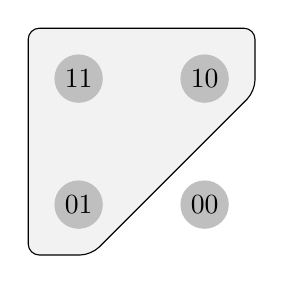
\begin{tikzpicture}[>=latex,scale=.8]
    
    % Possibilities
    \draw[opaque,rounded corners]
    (-1.8,0) -- (-1.8,1.8) -- (1.8, 1.8) -- (1.8,.8)
    -- (-.8,-1.8) -- (-1.8,-1.8) -- (-1.8,0);
    
    % Indices
    \draw (-1,1) node[index gray] (yy) {$11$};
    \draw (1,1) node[index gray] (yn) {$10$};
    \draw (-1,-1) node[index gray] (ny) {$01$};
    \draw (1,-1) node[index gray] (nn) {$00$};
  	
  	\end{tikzpicture}
  }
  \hspace{.2in}
  \subfigure[]{\label{inquisitive disjunction}
    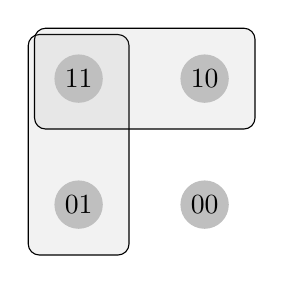
\begin{tikzpicture}[>=latex,scale=.8]
    
    % Possibilities
    \draw[opaque,rounded corners] (-1.8,1.7) rectangle (-.2, -1.8);
    \draw[opaque,rounded corners] (-1.7,1.8) rectangle (1.8, .2);

    % Indices
    \draw (-1,1) node[index gray] (yy) {$11$};
    \draw (1,1) node[index gray] (yn) {$10$};
    \draw (-1,-1) node[index gray] (ny) {$01$};
    \draw (1,-1) node[index gray] (nn) {$00$};
    
  	\end{tikzpicture}
  }
  \hspace{.2in}
  \subfigure[]{\label{inquisitive disjunction}
    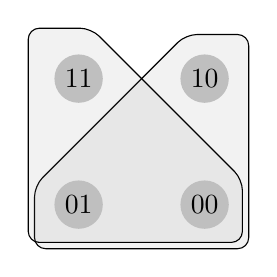
\begin{tikzpicture}[>=latex,scale=.8]
      
    % Possibilities
    \draw[opaque,rotate=180,rounded corners]
    (-1.7,0) -- (-1.7,1.7) -- (1.7, 1.7) -- (1.7,.7)
    -- (-.7,-1.7) -- (-1.7,-1.7) -- (-1.7,0);
    \draw[opaque,yscale=-1,xshift=-.1cm,yshift=-.1cm,rounded corners]
    (-1.7,0) -- (-1.7,1.7) -- (1.7, 1.7) -- (1.7,.7)
    -- (-.7,-1.7) -- (-1.7,-1.7) -- (-1.7,0);
    
    % Indices
    \draw (-1,1) node[index gray] (yy) {$11$};
    \draw (1,1) node[index gray] (yn) {$10$};
    \draw (-1,-1) node[index gray] (ny) {$01$};
    \draw (1,-1) node[index gray] (nn) {$00$};
  	
  \end{tikzpicture}
}
  \caption{Basic pictures}
  \label{fig:disjunction}
\end{figure}


%%%%%%%%%%%%%%%%%%%%%%%%%%%%%%%%%%%%%%%%%%%%%%%%%%%%%%%%%%%%%%%%%
%%%%%%%%%%%%%%%%%%%%%%%%%%%%%%%%%%%%%%%%%%%%%%%%%%%%%%%%%%%%%%%%%
%%%%%%%%%%%%%%%%%%%%%%%%%%%%%%%%%%%%%%%%%%%%%%%%%%%%%%%%%%%%%%%%%
%%%%%%%%%%%%%%%%%%%%%%%%%%%%%%%%%%%%%%%%%%%%%%%%%%%%%%%%%%%%%%%%%
%%%%%%%%%%%%%%%%%%%%%%%%%%%%%%%%%%%%%%%%%%%%%%%%%%%%%%%%%%%%%%%%%
%%%%%%%%%%%%%%%%%%%%%%%%%%%%%%%%%%%%%%%%%%%%%%%%%%%%%%%%%%%%%%%%%

\begin{figure}[h]
  \centering
  \subfigure[]{\label{partition}
    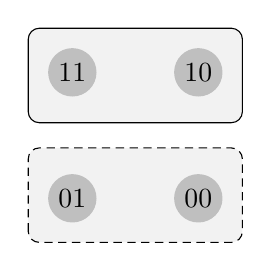
\begin{tikzpicture}[>=latex,scale=.8]
    
    % Possibilities
    \draw[opaque,rounded corners] (-1.7,1.7) rectangle (1.7, .2);
    \draw[opaque,counter,rounded corners] (-1.7,-1.7) rectangle (1.7, -.2);
    
    % Indices
    \draw (-1,1) node[index gray] (yy) {$11$};
    \draw (1,1) node[index gray] (yn) {$10$};
    \draw (-1,-1) node[index gray] (ny) {$01$};
    \draw (1,-1) node[index gray] (nn) {$00$};
  	
  	\end{tikzpicture}
  }
  \hspace{.2in}
  \subfigure[]{\label{inquisitive disjunction}
    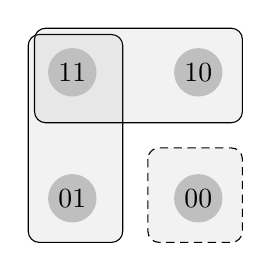
\begin{tikzpicture}[>=latex,scale=.8]
    
    % Possibilities
    \draw[opaque,rounded corners] (-1.7,1.6) rectangle (-.2, -1.7);
    \draw[opaque,rounded corners] (-1.6,1.7) rectangle (1.7, .2);
    \draw[opaque,counter,rounded corners] (.2,-.2) rectangle (1.7,-1.7);
    
    % Indices
    \draw (-1,1) node[index gray] (yy) {$11$};
    \draw (1,1) node[index gray] (yn) {$10$};
    \draw (-1,-1) node[index gray] (ny) {$01$};
    \draw (1,-1) node[index gray] (nn) {$00$};
    
  	\end{tikzpicture}
  }
  \hspace{.2in}
  \subfigure[]{\label{choice question}
    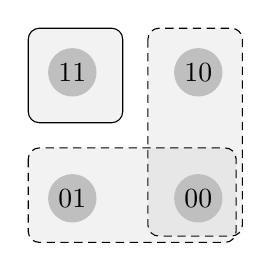
\begin{tikzpicture}[>=latex,scale=.8]
    
    % Possibilities
    \draw[opaque,rounded corners] (-1.7,1.7) rectangle (-.2, .2);
    \draw[opaque,counter,rounded corners] (.2,1.7) rectangle (1.7, -1.6);
    \draw[opaque,counter,rounded corners] (-1.7,-.2) rectangle (1.6, -1.7);
    
    % Indices
    \draw (-1,1) node[index gray] (yy) {$11$};
    \draw (1,1) node[index gray] (yn) {$10$};
    \draw (-1,-1) node[index gray] (ny) {$01$};
    \draw (1,-1) node[index gray] (nn) {$00$};
    
  	\end{tikzpicture}
  }
  \caption{Possibilities and counter-possibilities.}
  \label{fig:alternatives}
\end{figure}

%%%%%%%%%%%%%%%%%%%%%%%%%%%%%%%%%%%%%%%%%%%%%%%%%%%%%%%%%%%%%%%%%
%%%%%%%%%%%%%%%%%%%%%%%%%%%%%%%%%%%%%%%%%%%%%%%%%%%%%%%%%%%%%%%%%
%%%%%%%%%%%%%%%%%%%%%%%%%%%%%%%%%%%%%%%%%%%%%%%%%%%%%%%%%%%%%%%%%
%%%%%%%%%%%%%%%%%%%%%%%%%%%%%%%%%%%%%%%%%%%%%%%%%%%%%%%%%%%%%%%%%
%%%%%%%%%%%%%%%%%%%%%%%%%%%%%%%%%%%%%%%%%%%%%%%%%%%%%%%%%%%%%%%%%
%%%%%%%%%%%%%%%%%%%%%%%%%%%%%%%%%%%%%%%%%%%%%%%%%%%%%%%%%%%%%%%%%


\begin{figure}
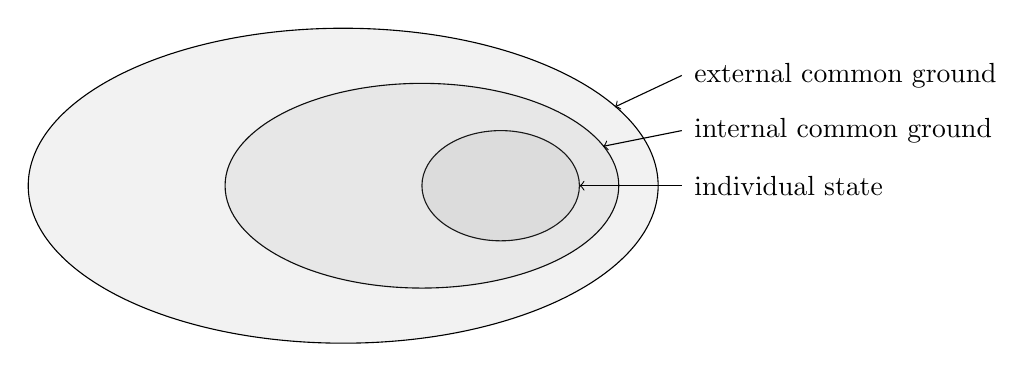
\begin{tikzpicture}

%ellipses
\draw[opaque] (0,0) ellipse (1cm and .7cm);
\draw[opaque] (-1,0) ellipse (2.5cm and 1.3cm);
\draw[opaque] (-2,0) ellipse (4cm and 2cm);

%labels
\draw[->] (2.3,0) node[right=1pt] {individual state} -- (1,0);
\draw[->] (2.3,.7) node[right=1pt] {internal common ground} -- (1.3,.5);
\draw[->] (2.3,1.4) node[right=1pt] {external common ground} -- (1.45,1);

\end{tikzpicture}
\caption{An individual information state, the internal, and the external common ground.}
\label{fig:common grounds}
\end{figure}

\end{document}
